% literature_review_clouds.tex
\chapter{Backgrounds about Clouds and Cloud Schemes}
\label{ch:literature_review_about_clouds}

In the following chapters, we will focus on clouds and cloud scheme. To begin with, the literature about clouds and cloud schemes are reviewed in this chapter. A general introduction about clouds is presented in \secref{sec:cld_intro}. \secref{sec:cloud_feedback} focuses on cloud feedback and our current understandings about how cloud feedback changes in response to climate change. The coupling between clouds and circulation is briefly introduced in \secref{sec:cld_circulation_coupling}. A short history of cloud scheme development is reviewed in \secref{sec:cld_scheme_history}. In \secref{sec:why_simple_cld_schem_in_isca} what kind of simple cloud scheme will be implemented in Isca and the reasons to do so are presented.

%\section{Clouds in observatixons}
%What are clouds and the distribution of clouds from observations

%\epigraph{\textit{Let's begin the scientific journey!}}{\textit{Qun Liu}, 2018}
%\section{Clouds in the observations}

%\section{Roles of clouds in climate system}
%\label{sec:chp2_role_of_clouds}
% Literature review about the role of clouds in climate system

\section{Introduction}
\label{sec:cld_intro}
%\subsection{Introduction}
Clouds usually cover more than half areas of the Earth at any given time \citep{Houze2014,Ramanathan1989}, which is supported by recent International Satellite Cloud Climatology Project (ISCCP)\index{ISCCP} H-series products \citep{Young2018}, as shown in \tabref{tab:statistics_cld_amt}. Although they vary among different regions, the cloud amounts are usually larger over ocean regions than over lands, as the ocean provides a abundance of water vapor.

\begin{table}[htp]
\centering
%\scriptsize
\caption{Statistics of the annually averaged total cloud amount for various regions, which are from the ISCCP H-series data sets \citep{Young2018} from 1984 to 2014.}
\vspace{0.5em}
\begin{tabular}{cccc}
	\toprule
	Region & Ocean & Land &  Total\\
	\midrule
	Global & 71.7 & 54.8 & 66.1 \\
	15$^\circ$S-15$^\circ$N&  62.4&  63.5& 62.6 \\
	15$^\circ$N-35$^\circ$N&  60.1&  46.6& 55.2\\
	15$^\circ$S-35$^\circ$S&  65.0&  48.3& 61.4\\
	35$^\circ$N-60$^\circ$N&  80.9&  64.6& 72.5 \\
	35$^\circ$S-60$^\circ$S&  84.0&  65.0& 83.5 \\
	60$^\circ$N-90$^\circ$N&  68.9&  62.0& 66.5\\
	60$^\circ$S-90$^\circ$S&  80.1&  44.3& 60.1 \\
	\bottomrule
\end{tabular}
\label{tab:statistics_cld_amt}
\end{table}

Clouds play a fundamental role in Earth's radiation budget and hydrological cycle. In general, clouds can reflect the sunlight (shortwave radiation) back into space and absorb the longwave radiation emitted from the surface and cloud-free atmosphere, part of which will return to the surface. In general, the net effect of cloud is to cool the earth comparing to the cloud-free conditions. According to \cite{Zelinka2017}, the net cooling effect of clouds is about 18 Wm$^{-2}$, which is roughly five times as large as the heating effect of doubling CO$_2$. Small changes in clouds can have a large impact on the climate energy balance due to balance between longwave and shortwave cloud effects. As a consequence, and not surprisingly, there are many studies focusing on the role of clouds in current climate or under climate change \citep[e.g.,][]{Cess1990intercomparison,Zelinka2017}.

% Therefore, even a small change of clouds could have large influence to the climate, that's one possible reason that why the cloud feedback is so important in climate system. 

%Clouds usually cover more than half areas of the Earth at any given time \citep{Houze2014} and play a fundamental role in Earth's radiation budget and hydrological cycle. In general, clouds can reflect the sunlight (shortwave radiation) back into space and absorb the longwave radiation emitted from the surface, part of which will return to the surface. In general, the net effect of cloud is to cool the earth comparing to the cloud-free conditions. According to \cite{Zelinka2017}, the net cooling effect of clouds is about 18 Wm$^{-2}$, which is roughly five times as large as the heating effect of doubling CO$_2$. Small changes in clouds can have a large impact on the climate energy balance due to balance between longwave and shortwave cloud effects. As a consequence, and not surprisingly, there are many studies focusing on the role of clouds under global warming \citep[e.g.,][]{Zelinka2017, Sherwood2020}.
% Therefore, even a small change of clouds could have large influence to the climate, that's one possible reason that why the cloud feedback is so important in climate system. 

%Besides interacting with radiation, clouds also couple with circulation \citep{Voigt2020review}.

Not only for the climatology, cloud responses to climate change have also attracted lots of attention. As described in detail in \secref{sec:cloud_feedback}, one important feature is cloud feedback, as it contributed a lot to the intermodel spread of the climate sensitivity of GCMs \citep{Ceppi2017, Sherwood2020}. In addition, clouds also have impact on the atmospheric circulation via their interactions with radiation \citep{Voigt2020review}, which can finally influence the regional climate, as reviewed in \secref{sec:cld_circulation_coupling}.

\section{Cloud feedback}
\label{sec:cloud_feedback}

\begin{figure}[ht]
	\centering
	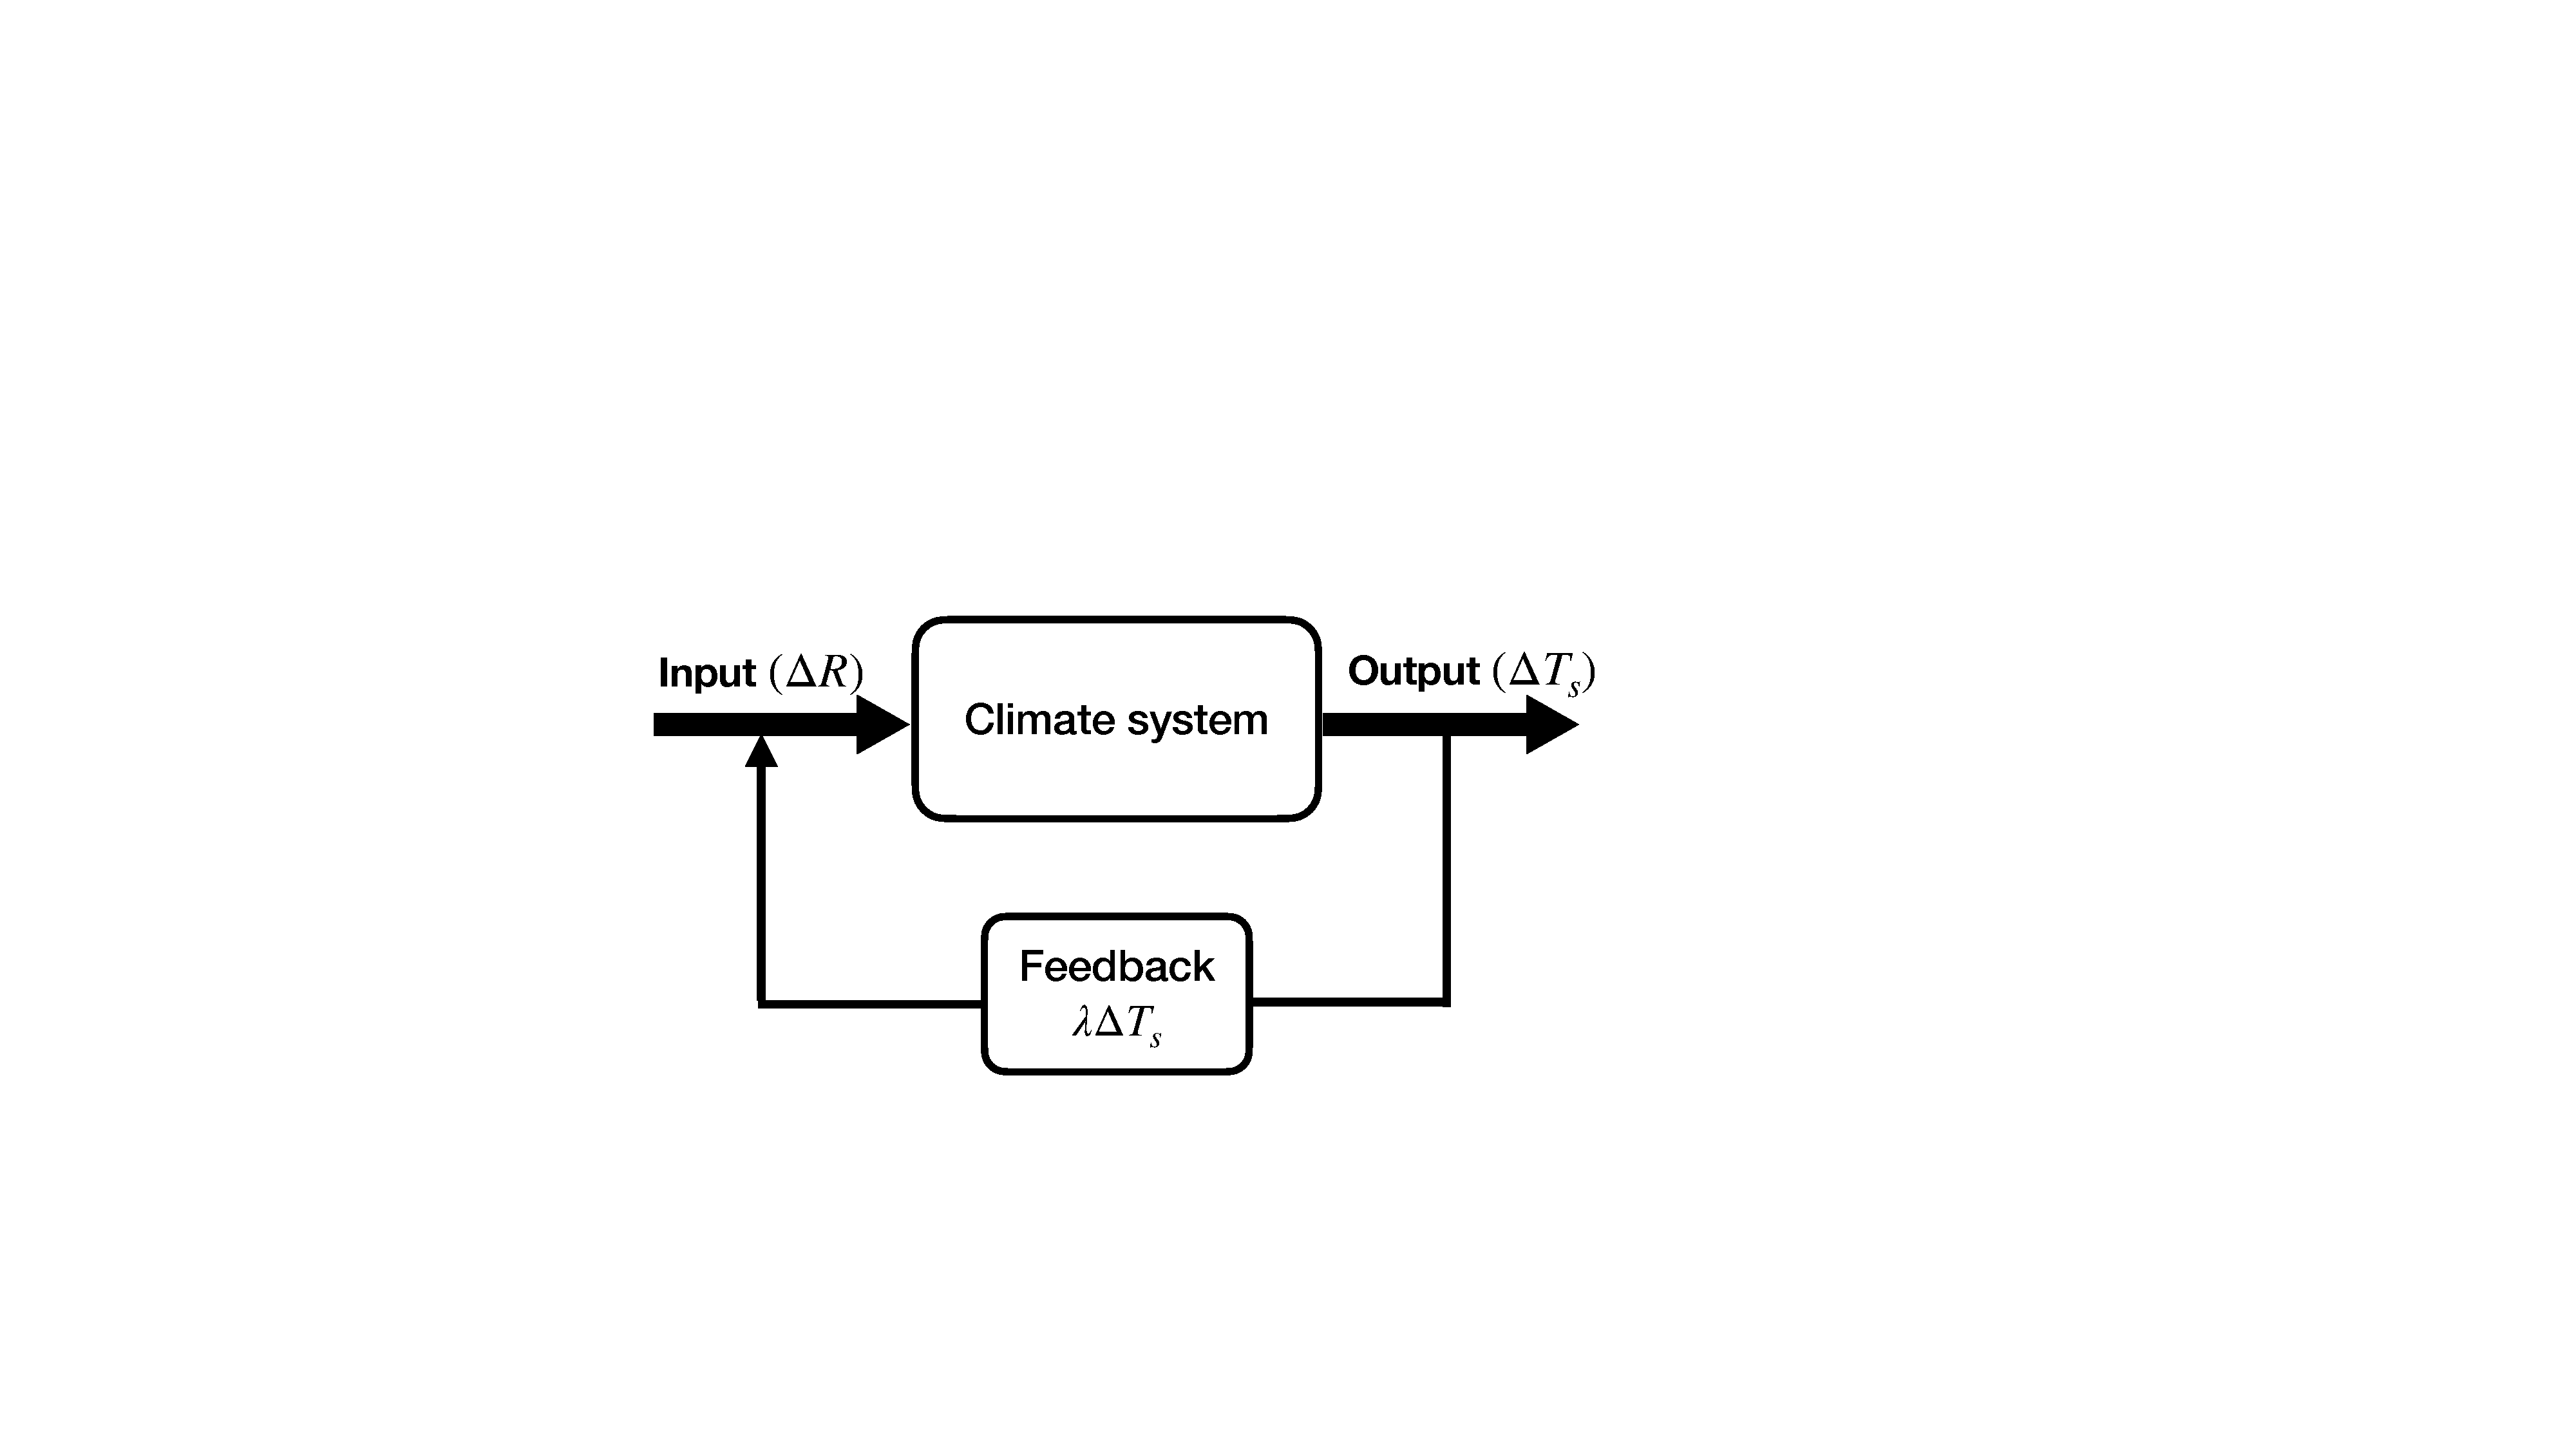
\includegraphics[width=0.6\linewidth]{{figs/literature_review/clim_system_feedback}.pdf}
	\caption{Schematic of feedback in climate system. $\Delta R$ is the input disturbance to the climate system, $\Delta T_s$ is the change of surface temperature and $\lambda$ denotes the climate feedback parameter.}
	\label{fig:schematic_climate_feedback}
\end{figure}

%What is feedback?
The idea of feedback\index{feedback} is taken from the control system, which is used to understand the system response to different forcings \citep{Stephens2005cloud}. As shown in \figref{fig:schematic_climate_feedback}, $\Delta R$ is the input to climate system, which can be seen as the radiative forcing produced by changing the content of CO$_2$ or aerosol, or by other factors such as volcanic eruption. Then many features in the climate system (such as surface temperature, specific humidity) would change in response to this forcing. In general, we select the surface temperature ($T_s$) as a key output variable. The change in surface temperature (i.e. $\Delta T_s$) can in turn impact the radiative balance at the top of the atmosphere (TOA)\index{top of the atmosphere (TOA)}. That is to say the output response is fed back to the system. The feedback parameter ($\lambda$, units Wm$^{-2}$K$^{-1}$) is a measure of the strength of the feedback. As introduced in \chapref{ch:polaramplification} there are many different feedbacks in the climate system, and here we focus on the ones related to clouds.

\begin{figure}[ht]
	\centering
	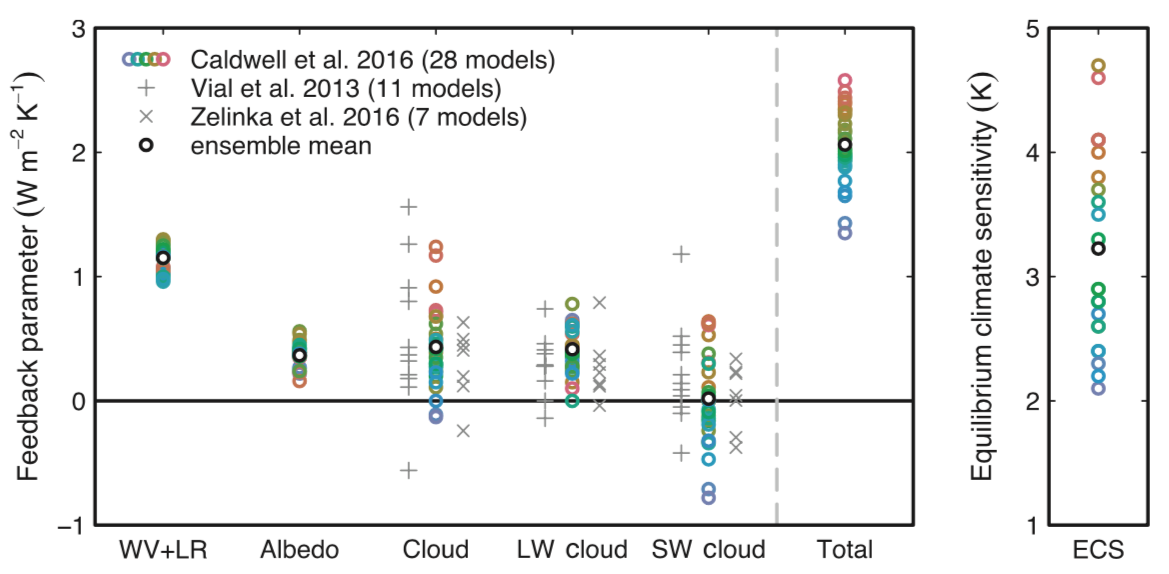
\includegraphics[width=1\linewidth]{{figs/literature_review/cloud_feedback_ceppi}.png}
	\caption{Strengths of individual global-mean feedbacks and equilibrium climate sensitivity (ECS) for CMIP5 models, derived from coupled experiments with abrupt quadrupling of CO$_2$ concentration. Circles are colored according to the total feedback parameter. The Planck feedback (mean value of -3.15 W m$^{-2}$ K$^{-1}$) is excluded from the total feedback parameter shown here. Adapted from \cite{Ceppi2017}.}
	\label{fig:cld_feed_back_ecs}
\end{figure}

Cloud feedback\index{cloud feedback} is the variation of cloud radiative forcing at the TOA in response to global warming. In the fifth assessment report of the Intergovernmental Panel on Climate Change (IPCC AR5), the sign of net cloud radiative feedback is likely positive with an estimate of 0.6 Wm$^{-2}$K$^{-1}$ \citep{stocker2013climate}, which, however, has a lot of uncertainties (-0.2 to 2 Wm$^{-2}$K$^{-1}$). As shown in Figure \ref{fig:cld_feed_back_ecs}, comparing to the water vapor, lapse rate and albedo feedbacks, cloud feedback is the largest uncertainty of simulated climate response to CO$_2$ foricng (i.e. climate sensitivity) in the general circulation models (GCMs) \citep{Ceppi2017}. Lots of efforts have been payed to investigate the possible reasons for the uncertainty of cloud feedbacks. For example, \cite{Webb2015} has proposed the Selected Process On/Off Klima Intercomparison Experiment (SPOOKIE) project, where the role of the convection has been accessed in the first phase of the project. They conclude that while parametrized convection influences the strength of the cloud feedbacks substantially in some models, other processes must also contribute substantially to the overall inter-model spread. In the second phase, the role of cloud scheme will be examined. For example, \cite{Geoffroy2017} found that the stratiform cloud scheme does play an important role in the spread of cloud feedback among the GCMs, both in stratocumulus regions and globally.

%, where the cloud fraction, cloud water content and effective cloud droplets radius are prescribed or will be diagnosed empirically.

A recent study by \cite{Sherwood2020} estimates that total cloud feedback is 0.45 Wm$^{-2}$K$^{-1}$ and the uncertainty (0.12 to 0.78 Wm$^{-2}$K$^{-1}$) is narrowed compared to the results from IPCC AR5. Nevertheless, the uncertainty of cloud feedback is still the largest one among all the feedback parameters (see Table 1 of \citealt{Sherwood2020}) and has no clear reduction from CMIP5 to CMIP6 (see Figure 4 of \citealt{Sherwood2020}).

%Cloud feedback decomposition? 
To fully understand cloud feedback is a challenging job, partly due to the diversity of clouds in climate system \citep{Zelinka2017}. For example, there are many different types of clouds, which are located at different locations and in different shapes or forms (such as liquid, ice or mixed phase), thus affecting the radiation in different ways. In addition, these clouds are usually controlled by different meteorological factors, therefore it is hard to predict the responses of clouds under climate change. Nevertheless, lots of efforts have been paid by previous studies to pin down the cloud feedback and here are some progresses. To make it clear, the cloud feedbacks are grouped into three categories: cloud amount, cloud altitude and cloud opacity feedbacks \citep{Zelinka2017}.

% cloud amount, cloud altitude, cloud opacity

\subsection{Cloud amount feedback}
% the cloud top of these clouds are usually high, meaning a low temperature at cloud top. 
The feedback induced by the cloud amount change is different for different cloud types. Specifically, the warming-induced increase of high, thin clouds usually leads to a positive feedback. The reason is that the optical depth of these high, thin clouds is typically small, thus having little impact on the shortwave radiation. However, the clouds can absorb the longwave radiation and thus constitute a strong greenhouse effect (XXXXXXX some reference). In contrast, the warming-induced increase in the amount of low clouds (opaque ones) brings a negative feedback as less sunlight can reach the surface, thus a cooling effects. These are the two typical cloud amount feedbacks.

Low clouds

marine low cloud changes are well described by reductions in low cloud fraction in response to local SST increases \citep[e.g.,][]{Rieck2012, Webb2013coupling, Qu2014, Bretherton2015, Brient2016,Ceppi2017relationship} and increases in low cloud fraction in response to increases in lower-tropospheric stability...This suggests that low cloud changes depend on local SST changes and remote effects that influence free tropospheric temperatures and hence lower-tropospheric stability \citep[e.g.,][]{Zhou2015,Zhou2016,Zhou2017,Andrews2018}. 

The formation and dissipation of low clouds are controlled by the differences between the supply of moisture from the surface and the mixing of relatively dry air above the boundary layer. The processes can be influenced by many large-scale meteorological factors, including sea surface temperature (SST), estimated inversion strength \citep[EIS;][]{Wood2006}, the relative humidity in the free troposphere, the strength of large-scale subsidence, warm/cold temperature advection and surface wind speed \citep{Scott2020}. The detailed effects are as follows:

\begin{enumerate}[label={(\arabic*)}]
    \item SST \\
    Warmer SST leads to the higher temperature and saturation water vapor pressure in the boundary layer, and can weaken the inversion strength if the temperature in the free troposphere remains constant. In this case, the in-cloud latent heating 
    \textcolor{red}{(I don't know why SST can influence the in-cloud latent heating?)} enhances the turbulance and entrainment of the drier air from aloft into the boundary layer, thus resulting in the reduction of cloudiness in low level.
    
    \item EIS \\
    Stronger EIS means more energy needed to mixing the relatively dry free-tropospheric air into the boundary layer and more moisture is trapped below the inversion layer, thereby favoring more low-level clouds.
    
    \item Subsidence \\
    Stronger subsidence can push down the boundary layer much lower and make the clouds lower and thinner, thereby supporting less low-level clouds.
    
    \item Moisture in free troposphere \\
    If the relative humidity in free troposphere is large, then the cloud-top entrainment drying is weaker, which thus favors more low-level clouds.
    
    
    At the same time, more free-tropospheric moisture emits more downwelling LW radiation, which can weaken cloud-top radiative-cooling and the overturning circulations that mix moisture up from the surface, thereby favoring less low-level cloud
    
    
    \item Warm/cold temperature advection\\
    %Stronger warm (cold) temperature advection in the boundary can lead to stronger upward (downward) latent heat flux
    Low-level advection from cold to warm SST brings relatively cool and dry air over warmer water, which triggers enhanced upward turbulent fluxes of heat and moisture from the sea surface, providing a strong source of moisture for cloud formation.
    
    Conversely, low-level airflow from warm to cold SST brings relatively warm and moist air over cooler water, which stabilizes the boundary layer and cuts off clouds from the surface moisture supply. 
    
    \item Surface winds\\
    Stronger winds increase evaporation from the sea surface and promote deepening of the boundary layer.
    
\end{enumerate}


\subsection{Cloud altitude feedback}

\subsection{Cloud opacity feedback}


\subsection{Role of cloud schemes in cloud feedback}

%Roles of parameterizations to the spread of cloud feedback among GCMs

Previous studies have shown that many parameterization schemes such as boundary layer and shallow convection can have impact on the spread of cloud feedbacks in GCMs \cite[e.g.,][]{Gettelman2012,Zhang2013CGILS,Sherwood2014spread}.
However, this inter-model spread did not decrease after the convective parametrizations being turn off \citep{Webb2015}, indicating that the difference in convection pramameterization schemes is not the main cause for inter-model spread of cloud feedback and other processes must also contribute substantially to the overall inter-model spread.

\cite{Zhang2013CGILS} proposed a mechanism to explain the positive subtropical low cloud feedback in climate models, in which the increased entrainment of dry air from the free troposphere into the boundary layer by parametrized convection in the warmer climate reduces low cloud amounts.

%For example, \cite{Sherwood2014spread} pointed out that the strength of convective mixing between the lower and middle tropical troposphere can explain about half of the variance in climate sensitivity estimated by GCMs. \cite{Zhang2013CGILS} showed that the differences in shallow convection schemes are causes of different cloud feedbacks in the models.

% The net cloud feedbacks can be considered as due to two opposing roles of surface-based PBL turbulence and shallow convection aided by cloud-top entrainment. \cite{Zhang2013CGILS} 

\cite{Geoffroy2017} implemented a range of diagnostic cloud schemes into two climate models (CAM4 and CSIRO-Mk3L) in lower troposphere, and found that roughly half of the multi-model spread in the cloud feedback in stratocumulus regions could be reproduced by changing the stratiform cloud scheme alone. In addition, they found that total water probability density function (PDF)-based schemes (see more in \secref{sec:PDF_cld_scheme}) tend to impose a positive low cloud feedback, while the stability dependent schemes tend to produce a negative feedback. These are similar to the findings of \cite{Qu2014}, in which they find the PDF-based schemes predict low cloud cover reduction in the stratocumulus regions, whereas most models employing schemes with stability dependent cloud fraction predict opposing changes in the same regions. In this case, it seems that stability dependence plays an important role in determining the sign of cloud feedback, which, however, does not fully determine the sign of cloud feedback, including in marine stratus regions \citep{Geoffroy2017}.

%\cite{Sherwood2010}

%\section{Cloud Radiative Effect and its feedback}

\section{Cloud-circulation coupling}
\label{sec:cld_circulation_coupling}

As introduced in previous section, in climate system clouds modulate the flow of energy by interacting with radiation, which then can have an impact on the circulation.

\cite{Voigt2020review}

\section{Cloud schemes}
\label{sec:cld_scheme_history}

\subsection{Overview}

\begin{figure}[ht]
	\centering
	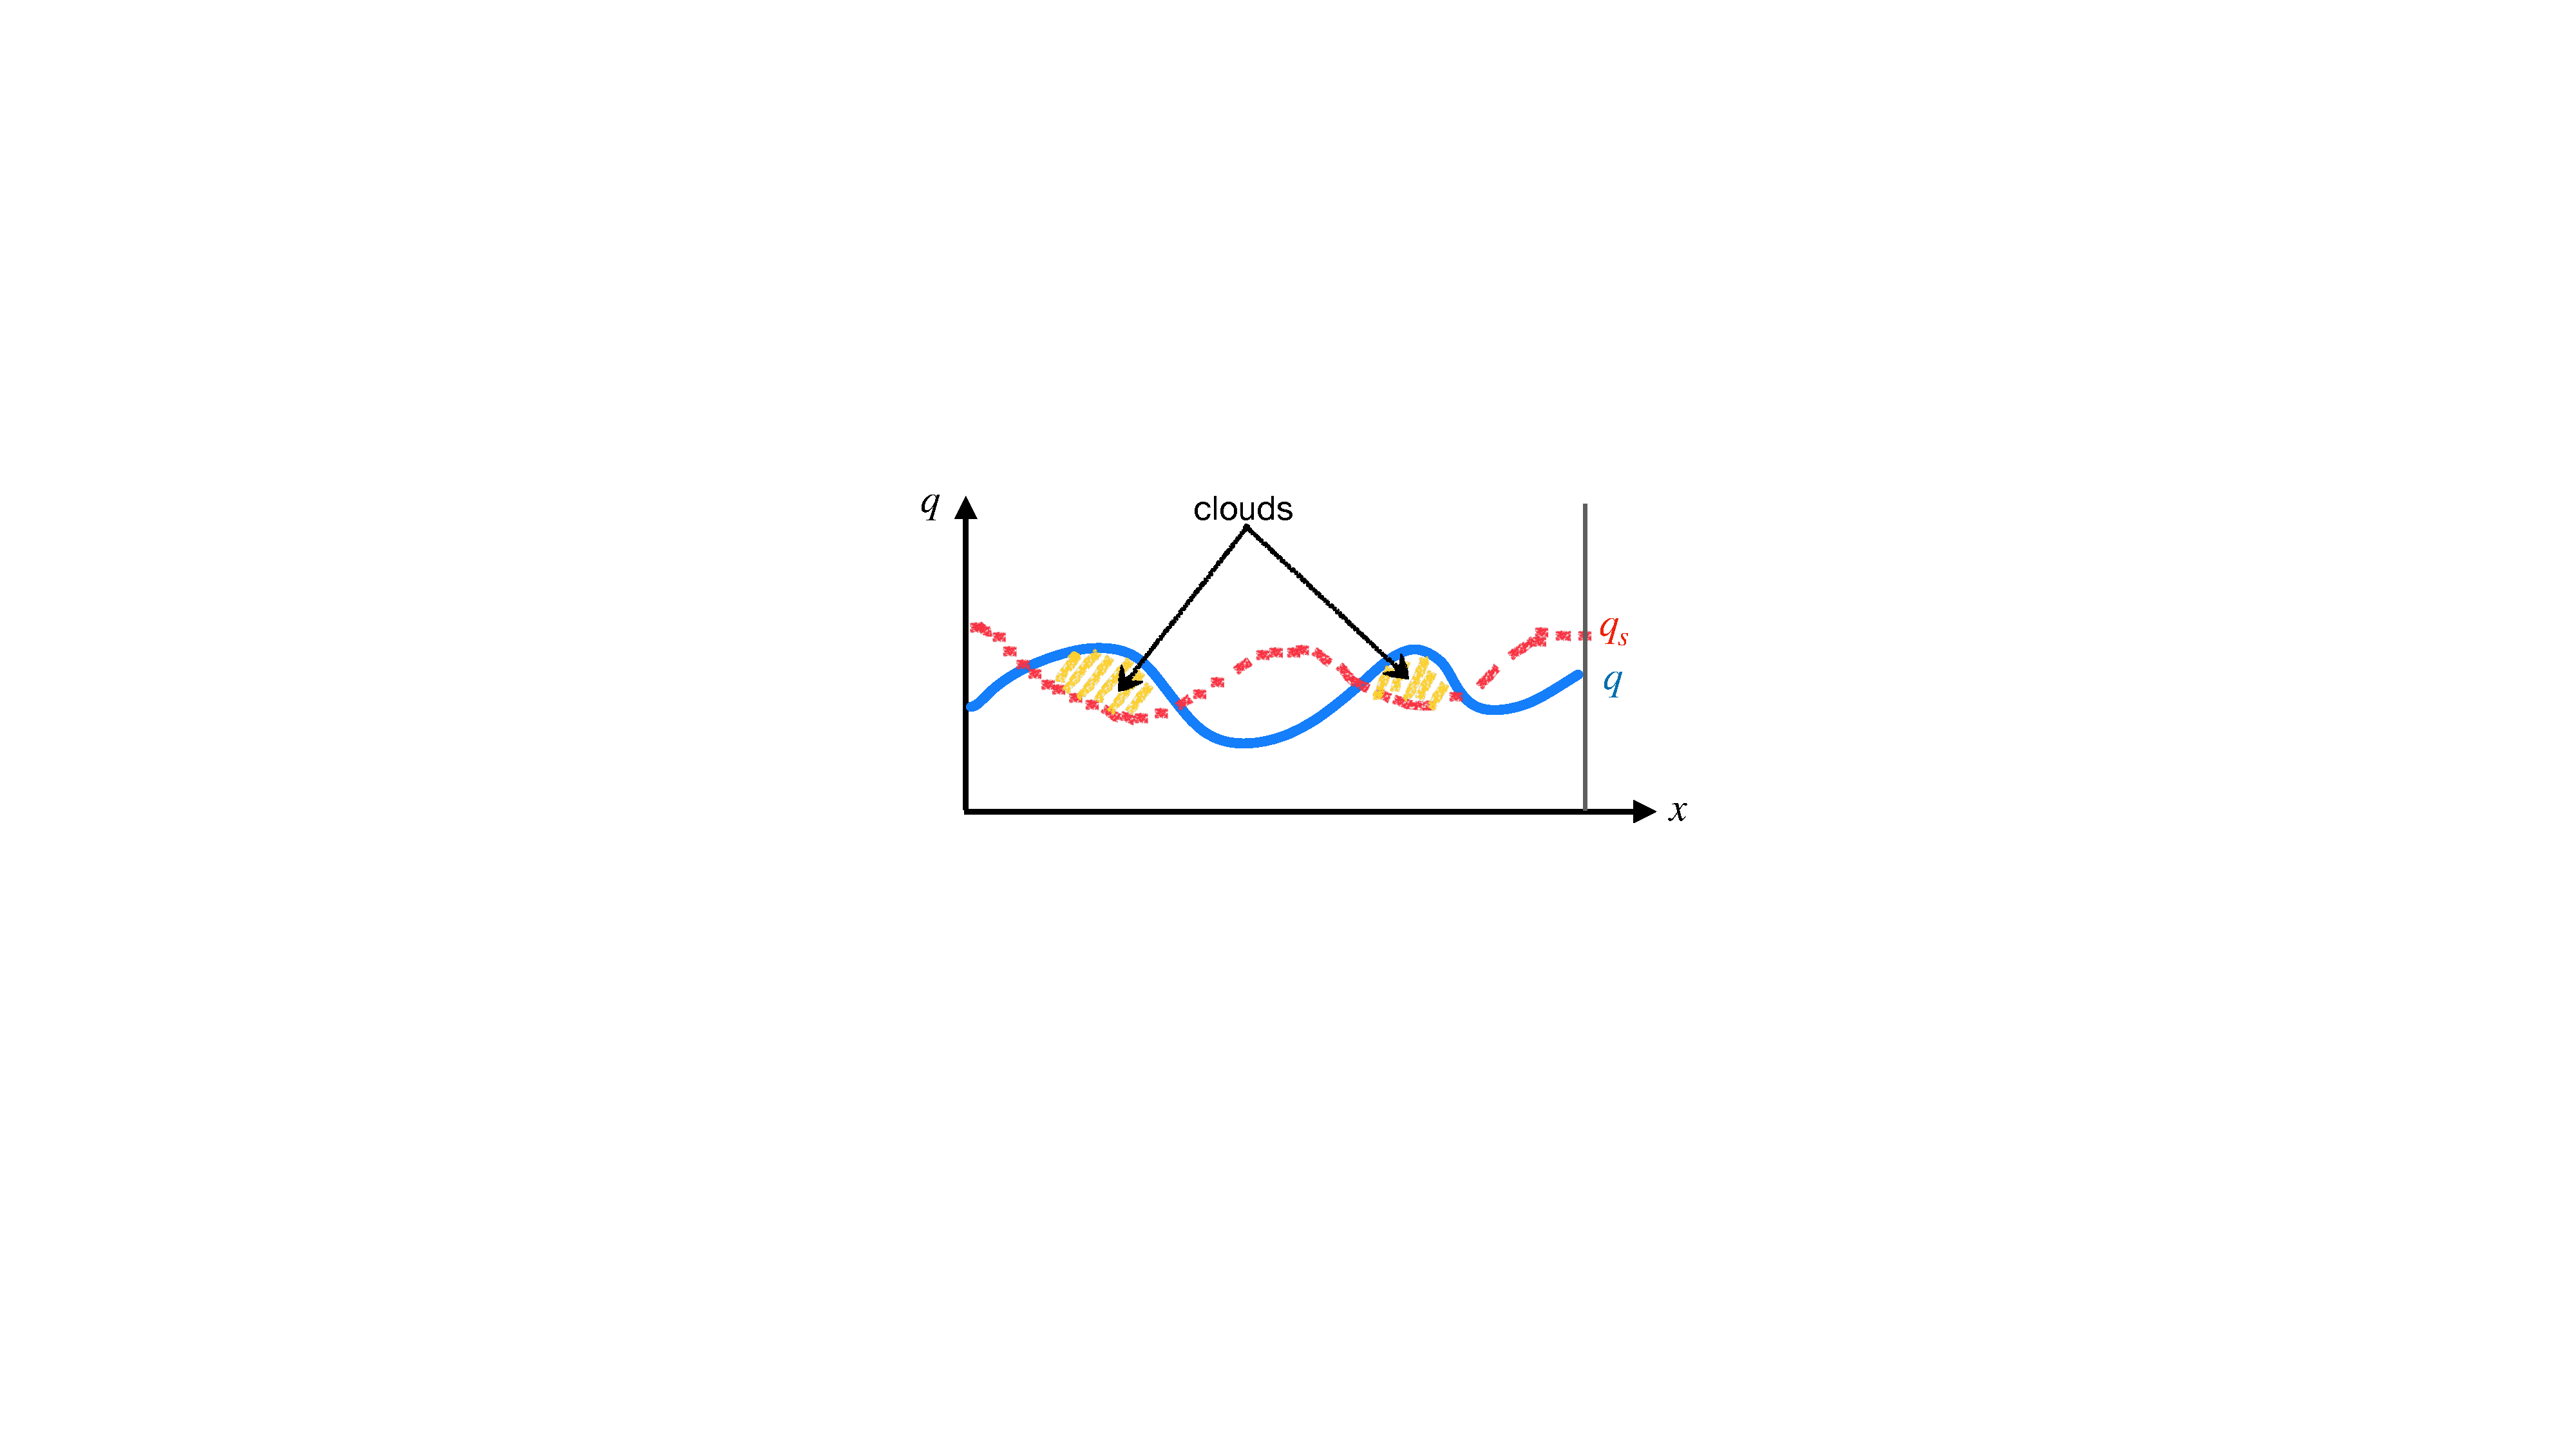
\includegraphics[width=0.8\linewidth]{{figs/literature_review/Schematic_partial_cloud_cover_in_gridbox}.pdf}
	\caption{Schematic showing that partial cloud cover in a grid box (1D) when temperature or humidity fluctuations exist. The blue line shows humidity and the red dashed line indicates saturation mixing ratio of the grid box. The shaded regions are cloudy parts as the humidity exceeds the saturation mixing ratio.}
	\label{fig:schematic_partial_clouds}
\end{figure}

At present the typical horizontal resolution of the GCMs is 50-200km, but the clouds usually involve the air motions in mesoscale and convective scale \citep{Houze2014}, which are usually in sub-grid scale both horizontally and vertically, implying that cloud processes are hard to be explicitly resolved by the GCMs. In this case, the ``parameterization" becomes a practical way to build cloud schemes. The parameterization is to represent the effects of the smaller-scale processes (turbulence, cloud microphysics, convection, etc.) in terms of the large-scale states (such as velocity, temperature, pressure, humidity) \citep{Randall2003}, which could be seen as a way to find potential relationships between the unknown and known variables \citep{Randall1989}.


\subsection{Relative humidity schemes}

Previous studies have investigated various ways to represent clouds in climate models. For example, \cite{Holloway1971} prescribed the clouds externally with climatological data without dynamic interplay with the other components of the model. Some early modelling studies made the assumption that a grid box in the model is either fully saturated or totally unsaturated. However, this assumption is not reasonable enough as the humidity can distribute unevenly within a grid box, suggesting that condensation can occur even the relative humidity is less than 100\%. A general idea is to link the cloud cover with the relative humidity, as one can expect that the amount of condensation would increase with the increase of mean humidity of the model grid box, which is the basis for some diagnostic methods.

Diagnostic schemes predict the cloudiness based on the model variables empirically or statistically. In these schemes, the clouds can be linked to atmospheric outputs such as relative humidity, vertical velocity and static stability, among which the linear relationship between cloud fraction against RH could be simplest one. For example, \cite{Smagorinsky1960} found empirically that non-convective cloud amount correlated with the average relative humidity in the respective layers (\figref{fig:Smagorinsky_RH_cld}), arguing that the non-precipitating condensation depend only on the accumulated history of vertical motion, which can be reflected by the humidity. \cite{Ricketts1973} obtained roughly linear relationship between cloud amount and observed relative humidity but commented that the relationship is somewhat indefinite.

Water vapor generally distributes heterogeneously in the grid box, so the averaged RH within a box should be less than 1 for a partial coverage of clouds. Previous studies usually adopt the critical relative humidity $RH_{crit}$ as the minimum threshold for clouds to form, which is often left as a free parameter that can be tuned during model development (e.g. \citealp{Hourdin2017,Kay2012,Mauritsen2012}). For example, \cite{Sundqvist1978} and \cite{Sundqvist1989} find that cloud fraction can be rewritten as a function of critical RH by assuming the water vapour is uniform distributed within the grid box. In general, $RH_{crit}$ decreases with height, but will vary according to different types of clouds. Although the $RH_{crit}$ doesn't have clear physical meaning, it can be used to modify the cloud amounts in different locations. For example, one can increase $RH_{crit}$ asymptotically to nearly unity to prevent the unrealistic circus clouds \citep{Sundqvist1989}. 

As a unique predictor, RH is very simple and useful to diagnose the cloudiness, and it is still widely used in GCMs \citep[e.g.,][]{Gordon1992,Park2014,Pope2000}. However, it is not valid for all the cases. As we can see, some studies also made use of other variables to diagnose the cloudiness. For instances, \cite{Xu1996} developed a semi-empirical scheme to determine the stratiform cloud fraction based on grid-averaged mixing ratio of condensate (cloud water and cloud ice) and RH. As for the scheme provided by \cite{Slingo1987}, both the RH and vertical velocity were taken into account, in which different empirical relations were used for different clouds including low, middle, high and convective clouds.

In summary, the methods based on relative humidity and other predictors are useful to diagnose the cloudiness, which ensures that the clouds can form before the grid box get saturated. One problem for the diagnostic methods is that in most cases the cloud condensate has to be diagnosed or prognosed via other methods \citep[e.g.,][]{Zhang2003, Park2014}, which could lead to some inconsistencies between cloud fraction and cloud condensate (e.g. \citealp{Gregory2002, Tompkins2005}).

\begin{figure}
	\vspace{-0.3cm}
	\centering
	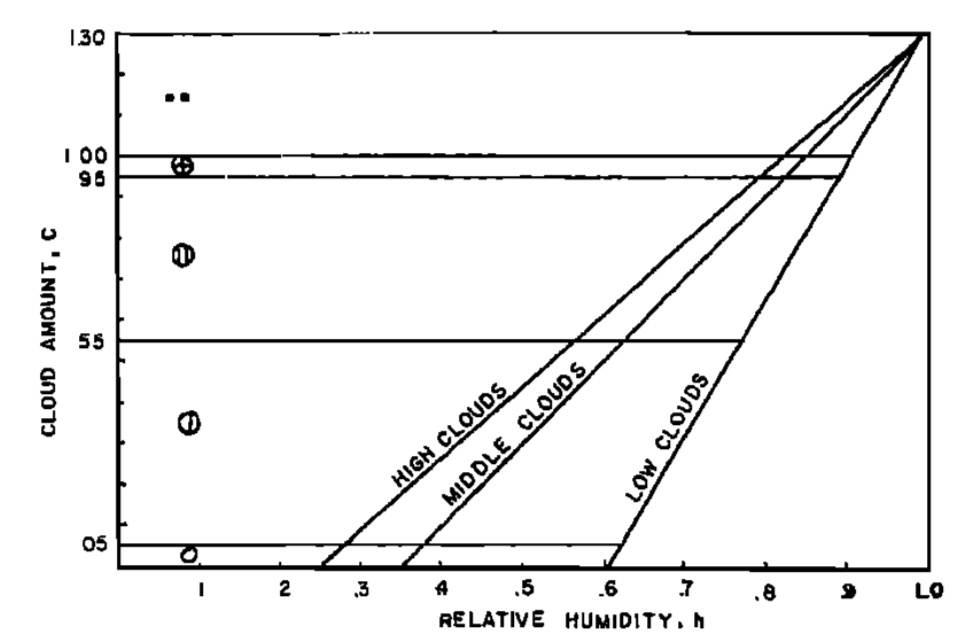
\includegraphics[width=0.6\linewidth]{{figs/literature_review/Smagorinsky1960}.png}
	\caption{Empirically determined relation of mean relative humidity $h$ in the layers 1000-800mb, 800-550mb and 550-300mb with cloud amount $c$ classed as low, middle and high clouds. Adapted from Figure 1 of \cite{Smagorinsky1960}.}
	\label{fig:Smagorinsky_RH_cld}
\end{figure}


\subsection{Statistical schemes}
\label{sec:PDF_cld_scheme}

In contrast, the prognostic approach \citep[e.g.,][]{Tiedtke1993} is to explicitly calculate the clouds related variables, such as cloud water content, in order to pursuing a unification of all clouds processes, which is more realistic in some degree and requires more physical basis and interactions with other parts of the models. Another widely used cloud prediction method is statistical scheme, in which the cloud fraction and in-cloud liquid water/ice are determined based on the assumed probability distributions of subgrid variability of thermodynamic properties. As the cloud related variables such as moisture and temperature are not the same everywhere but distributed randomly within the grid box, it is natural to assume that the cloud cover depends on the distribution of moisture, sometimes on the joint distribution of moisture and temperature. As shown in a very early work, \cite{Sommeria1977} gave up the assumption that a grid is either entirely saturated or unsaturated in the climate models and proposed the idea to use the statistical distribution of moisture within the grid box. For example, given the probability distribution function (PDF) of the total water ($q_t$ is the mixing ratio) in grid box, the cloud fraction ($CF$) can be calculated as 
\begin{equation}
    CF=\int_{q_s}^{\infty}\text{PDF}(q_t)\operatorname{d}q_t,
\end{equation}
and the cloud water content ($q_c$ is the mixing ratio of cloud water) is
\begin{equation}
    q_c=\int_{q_s}^{\infty}(q_t-q_s)\text{PDF}(q_t)\operatorname{d}q_t,
\end{equation}
where $q_s$ is the saturation mixing ratio in both formulations.

However, the shapes of subgrid-scale PDF of total water specific
humidity, saturation deficit, or a combined variable of liquid water and potential temperature are difficult to determine due to limit of observational data, so sometimes the model data are also used \citep{Bony2001}. Additionally, many different forms PDF have been proposed in the previous studies. For example, \cite{LeTreut1991} made use of the uniform distribution of total water in the grid box to calculate the clouds cover and liquid water content. Other symmetrical distributions, such as Gaussian distribution \citep{Sommeria1977}, triangular distribution \citep{Smith1990} and skewed distributions, such as lognormal distribution \citep{Bony2001} and beta distribution \citep{Tompkins2002}, have also been employed in numerical models. However, there are also some problems in the distributions. For example, the Gaussian distribution is unbounded, indicating that the maximum cloud condensate mixing ratio might approach infinity, and cloud cover is always large than zero \citep{Tompkins2002}. In general, complicated forms of the PDF need more parameters to fit. But due to the limitation of the data, it is possibly hard to validate the distributions. Linking the statistical cloud scheme to other physical processes seems a promising way to improve cloud simulations. For example, \cite{Qin2018} developed a Gaussian PDF cloud scheme with the PDF variance diagnosed from the turbulent
and shallow convective processes, which could improve the simulation of low marine clouds and alleviate double Intertropical Convergence Zone (ITCZ) problem \citep{Qin2018alleviated}.

The statistical cloud schemes may have better performance than the diagnostic ones, but considering the fact that there is no clouds scheme in Isca currently, it would be useful to implement the simple diagnostic schemes in Isca first, which can be seen as the first step to implemented a hierarchy of cloud schemes.

\subsection{Relationship between relative humidity and statistical schemes}

As discussed in previous section, one has to determine the expression of sub-grid variance (i.e. second order moment) or other higher-order moments in the statistical schemes. In doing so there are two general practices in current studies. The simple case is to use the time-invariant variance \citep[e.g.,][]{Sundqvist1978,Smith1990}, and the other approach is to employ time varying variance, which are usually obtained from other physical processes such as boundary layer scheme or shallow convection schemes \citep[e.g.,][]{Qin2018}. The second case usually provides a more realistic link between clouds and other physical processes \citep{Tompkins2002}. 

Note that there is no distinction between the RH schemes and statistical schemes, although they seem different in forms. As a matter of fact, if the subgrid variance in a statistical scheme is assumed to be time-invariant, it can be reduced to a RH scheme \citep{Tompkins2002,Tompkins2005}. The key is to link the variance with the critical relative humidity. That is to say, critical RH value can reflect the level of sub-grid variance in RH schemes \citep{Quaas2012}. Larger critical RH value means the lower subgrid variability and vice versa. For example, the \cite{Sundqvist1978} RH scheme can be derived by assuming a uniform distribution of total water mixing ratio within a grid box, in which the variance is assumed a constant fraction of the saturation water vapor mixing ratio, and this constant is associated with critical RH value (see Appendix A of \cite{Quaas2012} for a full derivation). Another example is the triangular distribution used by \cite{Smith1990} and \cite{Park2014}, they also obtain the equivalent RH formulation by assuming the variance is related to critical RH. As pointed by \cite{Tompkins2002}, the parameterizations such as \cite{Xu1996}, in which cloud fraction is related to RH and cloud condensate, can be viewed as manifestations of a statistical scheme although where the actual PDF of total water is not known. %, but the time-mean statistics of its integral are.

\section{Aims of the study}
\label{sec:why_simple_cld_schem_in_isca}
% This section introduce our goal to do for this phd study

The question then arises as to what a `simple' scheme is. One option would be to specify the PDF of total water within a grid box. Then, supposing that cloud formation occurs on saturation, one may be able derive a functional relation between mean cloud amount and mean relative humidity, supposing that the latter is what is predicted by the GCM from its predictions of specific humidity and temperature. \citet{Sundqvist1989} scheme was motivated this way, where the uniform distribution is adopted and variance of the distribution is assumed to be time-invariant \citep{Tompkins2005}. Although such a procedure is physically motivated it has two potential drawbacks. First, deciding on a distribution of humidity is somewhat arbitrary, or involves turbulence closure assumptions used in the stochastic model \citep{Sommeria1977,Tsang2018}. Second, translating the prediction of a probability distribution into a practical cloud model may be problematic, for there is in general no straightforward translation from a humidity probability distribution to an analytic formula connecting fractional cloud cover to relative humidity. 

Thus, here we chose another course by linking the cloud cover with the relative humidity ab initio. We explore two schemes, one with a piecewise linear relationship between cloud cover and relative humidity and the other with a square-root relationship, as in \citet{Sundqvist1989}. The various coefficients entering into these schemes are obtained empirically, comparing results with observations. We also use the scheme in an idealized GCM, Isca \citep{Vallis2018}, configured with a realistic distribution of continents to explore the geographical variability of the cloud schemes. Idealized models have a number of advantages in investigating physical processes, especially when set within a hierarchy connecting them to more comprehensive models \citep[e.g.,][]{Maher2018_hierarchies, Thomson2019}. We find that a relative-humidity scheme alone is unable to capture the subtropical low cloud distribution but that this can be readily improved by the addition of a scheme that takes into account inversion strength. Similarly, we find that in high-latitudes the cloud radiative effect is improved by the addition of a `freeze-dry' scheme. 

In its most complete form the scheme is able to capture the main features of clouds on Earth to a level of accuracy (in both geographical and seasonal variability) similar to that of other contemporary, and much more complicated, schemes in comprehensive climate models. It does so in a very transparent fashion and the dependence on parameters can be made explicit. And although we have implemented the scheme in a particular GCM it could easily be ported to others, either by an ab initio but straightforward implementation or by porting the code itself. 

% Idealised climate models can be used, amongst other things, to investigate how clouds impact the large-scale circulation, see  for a review. For example, using the cloud locking approach or investigating the behaviour of a process in the absence of clouds, such as the Isca model that does not have clouds or water vapour feedbacks. For our purpose, the scheme should be simple enough to facilitate understanding of the role of clouds in the dynamics of climate variability and climate change, but complex enough to be able to capture the main features of clouds on Earth, comparable to that of other contemporary (and more complicated) climate models.

% We organize the paper as follows. Section 2 provides a description of the simple cloud scheme, SimCloud, including the methods to parameterize the cloud fraction and specify other needed physical parameters, such as the effective radius of cloud droplets and in-cloud condensate content. (Some of the choices and parameters used come from the experiments and observations described in later sections, but for clarity the cloud scheme is described first.) Section 3 describes the model and experimental configurations as well as the data sets used in this study. In Sect. 4 we compare the simulated cloud properties with observations, with an emphasis on the CRE. A discussion and conclusions are presented in Sect. 5.